
\documentclass[final,hyperref={pdfpagelabels=false}]{beamer}

\usepackage[orientation=portrait,size=a0,scale=1.4]{beamerposter} % Use the beamerposter package for laying out the poster with a portrait orientation and an a0 paper size

\usetheme{I6pd2} % Use the I6pd2 theme supplied with this template

\usepackage[english]{babel} % English language/hyphenation

\usepackage{amsmath,amsthm,amssymb,latexsym} % For including math equations, theorems, symbols, etc

%\usepackage{times}\usefonttheme{professionalfonts}  % Uncomment to use Times as the main font
%\usefonttheme[onlymath]{serif} % Uncomment to use a Serif font within math environments

\boldmath % Use bold for everything within the math environment

\usepackage{booktabs} % Top and bottom rules for tables

\graphicspath{{figures/}} % Location of the graphics files

\usecaptiontemplate{\small\structure{\insertcaptionname~\insertcaptionnumber: }\insertcaption} % A fix for figure numbering

%----------------------------------------------------------------------------------------
%	TITLE SECTION 
%----------------------------------------------------------------------------------------

\title{\huge A New Class of Cosmologically viable $f(R)$ models} % Poster title

\author{Rohin Kumar Y} % Author(s)

\institute{Department of Physics \& Astrophysics, University of Delhi} % Institution(s)

%----------------------------------------------------------------------------------------
%	FOOTER TEXT
%----------------------------------------------------------------------------------------

\newcommand{\leftfoot}{http://www.github.com/rohinkumar} % Left footer text

\newcommand{\rightfoot}{yrohinkumar@gmail.com} % Right footer text

%----------------------------------------------------------------------------------------

\begin{document}

\addtobeamertemplate{block end}{}{\vspace*{2ex}} % White space under blocks

\begin{frame}[t] % The whole poster is enclosed in one beamer frame

\begin{columns}[t] % The whole poster consists of two major columns, each of which can be subdivided further with another \begin{columns} block - the [t] argument aligns each column's content to the top

\begin{column}{.02\textwidth}\end{column} % Empty spacer column

\begin{column}{.465\textwidth} % The first column
%
%%----------------------------------------------------------------------------------------
%%	OBJECTIVES
%%----------------------------------------------------------------------------------------
%
\begin{block}{Background}

\begin{enumerate}
	\item Alternative gravity models - to resolve problems of Cosmology?
	%\item $f(R)$ theories - toy-models in exploring alternative gravity cosmologies.
	\item $\Lambda CDM$ considered only `viable' Cosmology  despite unknown ``Dark" entities
	\item $f(R)$ theories are generally studied to be fit as the possible candidates for either dark energy, dark matter or both - but their efficacy is judged based on fit with $\Lambda CDM$ only
	%\item Modified gravity models have been successful in explaining the flat rotation curves of galaxies.
\end{enumerate}

\end{block}

%----------------------------------------------------------------------------------------
%	INTRODUCTION
%----------------------------------------------------------------------------------------
            
\begin{block}{Motivation}

\begin{itemize}
\item No one definitive $f(R)$ model that possibly satisfies all the required criteria to be an alternative to $\Lambda$CDM model.
\item Their viability is always judged based on it's ability to reproduce scale factor evolution as predicted by $\Lambda$CDM model.
\item idea! - ``Designer" approach to $f(R)$ with alternative models of scale factor evolution!
\item To explore the possible new viable models assuming the universe is evolving with linear scale factor (at least during matter domination).
\end{itemize}

\end{block}

%----------------------------------------------------------------------------------------
%	MATERIALS
%----------------------------------------------------------------------------------------

\begin{block}{Linearly Coasting Universe?}

\begin{columns} % Subdivide the first main column
\begin{column}{.40\textwidth} % The first subdivided column within the first main column
\begin{itemize}
	\item A linearly coasting $a(t)$ is as good a fit to Supernovae data as $\Lambda CDM$\cite{nielsen2015marginal}
	\item Doesn't need inflation \& ``Dark" stuff e.g. empty open Universe (Milne)
	\item $a\propto t$ - pioneering work done by Daksh Lohiya et al.\cite{gehlaut2002freely}
	\item Recent proposals include $R_h=ct$ model\cite{melia2012rh}
\end{itemize}
\end{column}

\begin{column}{.60\textwidth} % The second subdivided column within the first main column
\centering
\begin{figure}
\includegraphics[width=0.75\linewidth]{"./figures/Sarkar_fig3a"}
\caption{Linearly Coasting vs. $\Lambda CDM$\cite{nielsen2015marginal}}
\end{figure}
\end{column}
\end{columns} % End of the subdivision

\end{block}

%----------------------------------------------------------------------------------------
%	METHODS
%----------------------------------------------------------------------------------------

\begin{block}{Basic $f(R)$ Theory}
In the metric formalism of $f(R)$ theory. We write the action as 
\begin{equation}
S={1 \over 2\chi} \int d^4x\sqrt{-g}f(R)+S_{matter}
\end{equation}
Here $\chi=8\pi G$ where `G' is universal gravitational constant.
Extremizing the action w.r.t $\delta g^{\alpha\beta}$ to write $\delta S=0$

\begin{equation}
	f'(R)R_{\mu\nu}-
\frac{1}{2}f(R)g_{\mu\nu}
-(\nabla_\mu\nabla_\nu-g_{\mu\nu}\square)f'(R)=\chi T_{\mu\nu}
\label{gfe}
\end{equation}

Starting with the FLRW metric element 
\begin{equation}
ds^2=-dt^2+a^2(t)\left(\dfrac{dr^2}{1-\kappa r^2}+r^2(d\theta^2+\sin^2\theta d\phi^2)\right)
\end{equation}

for a generic $f(R)$ model, we get modified Friedmann equations as

\begin{equation}
H^2+\dfrac{\kappa}{a^2}=\dfrac{1}{3f'(R)}\left[\chi \rho+\dfrac{Rf'(R)-f(R)}{2}-3Hf''(R)\dot{R}\right]
\label{modfrw1}
\end{equation}

and 

\begin{multline} 
2\dot{H}+3H^2+\dfrac{\kappa}{a^2}=-\dfrac{1}{f'(R)}\bigg[\chi P+2H\dot{R}f''(R)+\\
\dfrac{f(R)-Rf'(R)}{2}+\ddot{R}f''(R)+\dot{R}^2f'''(R)\bigg]\label{modfrw2}
\end{multline}

\end{block}

%----------------------------------------------------------------------------------------
%	Approach
%----------------------------------------------------------------------------------------

\begin{block}{`Designer' Approach }
\begin{figure}
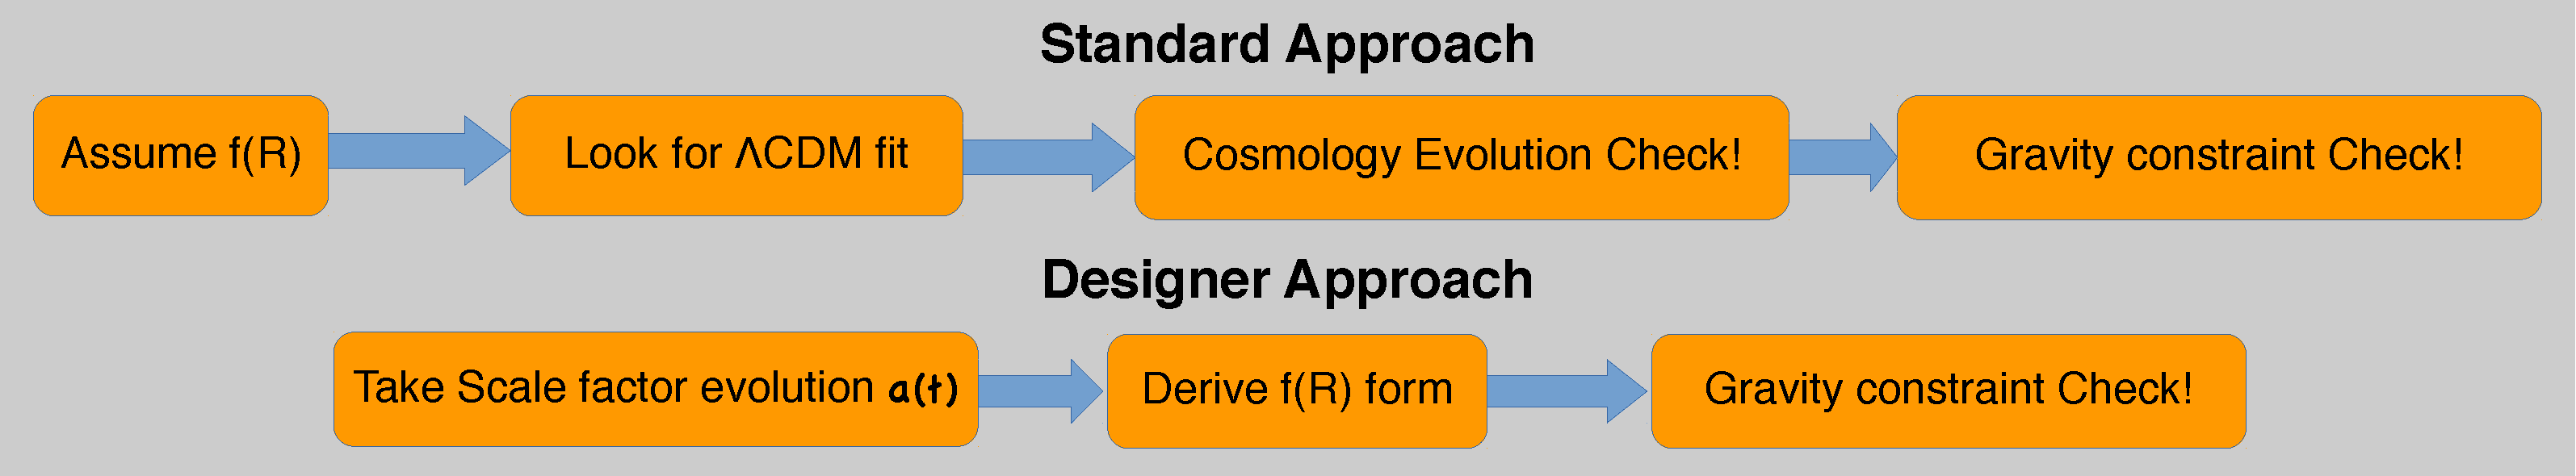
\includegraphics[width=1.0\linewidth]{designer_vs_std}
%\caption{Approach for new `viable' $f(R)$}
\end{figure}

\end{block}

%----------------------------------------------------------------------------------------

\end{column} % End of the first column

\begin{column}{.03\textwidth}\end{column} % Empty spacer column
% 
\begin{column}{.465\textwidth} % The second column
%
%%----------------------------------------------------------------------------------------
%%	RESULTS
%%----------------------------------------------------------------------------------------
%
%\begin{block}{Results: Table}
%
%\begin{itemize}
%\item Ased Aliquet Luctus Lectus
%\end{itemize}
%
%\begin{table}
%\begin{tabular}{l l l}
%\toprule
%\textbf{Treatments} & \textbf{Response 1} & \textbf{Response 2}\\
%\midrule
%Treatment 1 & 0.0003262 & 0.562 \\
%Treatment 2 & 0.0015681 & 0.910 \\
%Treatment 3 & 0.0009271 & 0.296 \\
%\bottomrule
%\end{tabular}
%\caption{Table caption}
%\end{table}
%
%\begin{itemize}
%\item Sollicitudin Vel Orci
%\item Maecenas Ultricies Feugiat Velit Non Mattis.
%\end{itemize}
%
%\begin{table}
%\begin{tabular}{l l l}
%\toprule
%\textbf{Treatments} & \textbf{Response 1} & \textbf{Response 2}\\
%\midrule
%Treatment 1 & 0.0003262 & 0.562 \\
%Treatment 2 & 0.0015681 & 0.910 \\
%Treatment 3 & 0.0009271 & 0.296 \\
%\bottomrule
%\end{tabular}
%\caption{Table caption}
%\end{table}
%     
%\end{block}
%
%%------------------------------------------------
%
\begin{block}{$f(R)$ of a Linearly Coasting Universe}
For a linearly coasting scale factor we have 
\begin{equation}
a(t)\propto t \implies a(t)=t/t_0 \implies H(t)={1 \over t}~~~\&~~~H_0={1\over t_0}
\end{equation}

For FLRW metric Ricci scalar is
\begin{equation}
R=6(2H^2+\dot{H}+\kappa/a^2) 
\end{equation}

%\subsection{For $\kappa=0$:}
\textbf{For $\kappa=0$:}
Assuming a flat Universe, we have 

\begin{equation}
R=6(2H^2+\dot{H}) = {6 \over t^2} = 6H^2 \implies H=\sqrt{R/6}\label{Rk0}
\end{equation}

%Using this expression we can convert the modified Friedmann equations \eqref{modfrw1} and \eqref{modfrw2} into functions of $R$.

This leads us to 
\begin{equation}
R^2f''-f/2+\chi\rho=0\label{fR1k0}
\end{equation}

\begin{equation}
2R^3f'''+R^2f''-Rf'+{3 \over 2}f+3\chi P =0\label{fR2k0}
\end{equation}

Assuming the equation of state $w=P/\rho$, we get a $2^{nd}$ order differential equation

\begin{equation}
f''-{1\over 2R^2}f+{\alpha R^{{3 \over 2}(1+w)}\over R^2}=0\label{difffRk0}
\end{equation}

As one can quickly identify, the numerator in the last term is nothing but the matter/radiation density 

\begin{equation}
\rho = {\rho_0 a_0^3 \over a^3} = {\rho_0 t_0^3 \over t^3} \implies \rho = \alpha R^{{3 \over 2}(1+w)}
\end{equation}
where $\alpha = \chi\rho_0 t_0^3= {8\pi G\rho_0 \over H_0^3}$

Solving \eqref{difffRk0} we get a possibly viable form for $f(R)$

\begin{equation}
f(R)=-{4\alpha \over 1 + 3 w (4 + 3 w)} R^{{3 \over 2}(1+w)}+C_1R^{(\sqrt{3}+1)/2}+C_2R^{(-\sqrt{3}+1)/2}\label{fR1}
\end{equation}
\begin{itemize}
	\item This form is a potentially viable $f(R)$ with constants $C_1$, $C_2$ and $\rho_0$(and hence $\alpha$) need to be constrained using observational data.
	\item Since we are primarily interested in late-time acceleration as observed by supernovae data we can assume the case of matter dominated era  $P_{matter}=0$ making $w=0$ in \eqref{fR1} giving us
\end{itemize}

\begin{equation}
f(R)=-4\alpha R^{{3 \over 2}}+C_1R^{(\sqrt{3}+1)/2}+C_2R^{(-\sqrt{3}+1)/2}\label{fR2}
\end{equation}

%For the sake of completion, if the Universe was primarily radiation dominated ($w=1/3$)at late times we get 
%
%\begin{equation}
%f(R)=-2/3\alpha R^2+C_1R^{(\sqrt{3}+1)/2}+C_2R^{(-\sqrt{3}+1)/2}\label{fR3}
%\end{equation}
%
%%\subsection{For $\kappa>0$:}
%\textbf{For $\kappa>0$:}
%In case of the closed universe, we have $\kappa/a^2 = 1/t^2$ for linear coasting. This gives us
%\begin{equation}
%R=6(2H^2+\dot{H}+\kappa/a^2) = 12/t^2 = 12H^2 \implies H =\sqrt{R/12}
%\end{equation}
%Rest of the equations follow this definiton of Ricci scalar giving rise to
%\begin{equation}
%R^2f''+Rf'-f+2\chi\rho=0
%\end{equation}
%\begin{equation}
%R^3f'''+R^2/2f''-{3 \over 2}Rf'+{3 \over 2}f+3\chi P = 0
%\end{equation}
%
%Solving these two equations, we have a simpler $1^{st}$ order differential equation unlike \eqref{difffRk0} as
%\begin{equation}
%f'-{1 \over R}f+{\alpha \over 2}{R^{{3 \over 2}(1+w)} \over R}=0
%\end{equation}
%
%Solving this we get 
%\begin{equation}
%f(R)=C_1R-{2\alpha \over (1 + 3 w)} R^{{3 \over 2}(1 + w)}
%\end{equation}
%
%For matter dominated universe, we have 
%
%\begin{equation}
%f(R)=C_1R-2\alpha R^{{3 \over 2}}
%\end{equation}
%
%In case of radiation dominated Universe, we have
%\begin{equation}
%f(R)=C_1R-\alpha R^2
%\end{equation}
%
%These are familar forms of $f(R)$ however they still need to be explored in the context of linear coasting model.

%\subsection{For $\kappa < 0$:}
%\textbf{For $\kappa<0$:}
%Unfortunately in the open Universe case, $\kappa/a^2 = -1/t^2$ gives 
%
%\begin{equation}
%R=6(2H^2+\dot{H}+\kappa/a^2) = 0
%\end{equation}


\end{block}
%
%%----------------------------------------------------------------------------------------
%%	CONCLUSION
%%----------------------------------------------------------------------------------------

\begin{block}{Conclusions \& Future Work}

\begin{itemize}
\item Assuming a linearly coasting scale factor, we derived a potentially new `viable' forms of $f(R)$.
\item While some forms may look familar, they need to be re-evaluated in the light of linear coasting.
\item Constraining these $f(R)$ models with Cosmological observations 
\begin{itemize}
	\item linear growth rate of structures
	\item gravitational weak lensing 
	\item CMB and structure formation theories
	\item weak field limit from the solar system tests
	\item gravitational wave observations
\end{itemize}

\item These areas are to be explored in the subsequent work(s).
\end{itemize}

\end{block}

%%----------------------------------------------------------------------------------------
%%	REFERENCES
%%----------------------------------------------------------------------------------------

\begin{block}{References}
        
\nocite{*} % Insert publications even if they are not cited in the poster
\small{\bibliographystyle{acm}
\bibliography{IAGRG_poster_ref}}

\end{block}

%%----------------------------------------------------------------------------------------
%%	ACKNOWLEDGEMENTS
%%----------------------------------------------------------------------------------------
%
%\begin{block}{Acknowledgments}
%
%\begin{itemize}
%\item Nam mollis tristique neque eu luctus. Suspendisse rutrum congue nisi sed convallis. Aenean id neque dolor. Pellentesque habitant morbi tristique senectus et netus et malesuada fames ac turpis egestas.
%\end{itemize}
%
%\end{block}

%----------------------------------------------------------------------------------------
%	CONTACT INFORMATION
%----------------------------------------------------------------------------------------

%\setbeamercolor{block title}{fg=black,bg=orange!70} % Change the block title color
%
%\begin{block}{Contact Information}
%
%\begin{itemize}
%\item Web: \href{http://www.github.com/rohinkumar}{http://www.github.com/rohinkumar}
%\item Email: \href{mailto:yrohinkumar@gmail.com}{yrohinkumar@gmail.com}
%\item Phone: +91 9818092877
%\end{itemize}

%\end{block}

%%----------------------------------------------------------------------------------------
%
\end{column} % End of the second column

\begin{column}{.015\textwidth}\end{column} % Empty spacer column

\end{columns} % End of all the columns in the poster

\end{frame} % End of the enclosing frame

\end{document}